%
% Modelo de trabalho acadêmico (Teses, Dissertações, TCC)
% Documento principal
%
% Centro Federal de Educação Tecnológica de Minas Gerais - CEFET-MG
% Autor: Cristiano Fraga G. Nunes <cfgnunes@gmail.com>
%
% Projeto hospedado em: https://github.com/cfgnunes/latex-cefet-mg
%
%
% Informações:
%   Codificação utilizada: UTF-8
%   Tamanho da tabulação: 4 (espaços)


\documentclass[oneside]{abntex2-cefetmg}            % Imprimir apenas frente
%\documentclass[doubleside]{abntex2-cefetmg}        % Imprimir frente e verso

% Importações de pacotes
\usepackage[portuguese, onelanguage, lined, boxed, commentsnumbered, algoruled]{algorithm2e}                % Escrever algoritmos
\usepackage[alf, abnt-emphasize=bf, bibjustif, recuo=0cm, abnt-etal-cite=2, abnt-etal-list=0]{abntex2cite}  % Citações padrão ABNT
\usepackage[utf8]{inputenc}                         % Acentuação direta
\usepackage[T1]{fontenc}                            % Codificação da fonte em 8 bits
\usepackage{graphicx}                               % Inserir figuras
\usepackage{amsfonts, amssymb, amsmath}             % Fonte e símbolos matemáticos
\usepackage{booktabs}                               % Comandos para tabelas
\usepackage{verbatim}                               % Texto é interpretado como escrito no documento
\usepackage{multirow, array}                        % Múltiplas linhas e colunas em tabelas
\usepackage{indentfirst}                            % Endenta o primeiro parágrafo de cada seção.
\usepackage{microtype}                              % Para melhorias de justificação?
\usepackage{float}                                  % Utilizado para criação de floats
\usepackage{icomma}                                 % Uso de vírgulas em expressões matemáticas
\usepackage{palatino}                               % Usa a fonte Palatino
%\usepackage{times}                                 % Usa a fonte Times
%\usepackage{lmodern}                               % Usa a fonte Latin Modern
%\usepackage{color, colortbl}                       % Comandos de cores
%\usepackage{listings}                              % Importação de códigos fonte
%\usepackage[bottom]{footmisc}                      % Mantém as notas de rodapé sempre na mesma posição
%\usepackage{subfig}                                % Posicionamento de figuras
%\usepackage{scalefnt}                              % Permite redimensionar tamanho da fonte
%\usepackage{lscape}                                % Permite páginas em modo "paisagem"
%\usepackage{picinpar}                              % Dispor imagens em parágrafos

% Inclui o preâmbulo do documento
%
% Documento: Preâmbulo
%

\titulo{Otimizando Desempenho de \textit{Front-end} em \textit{Websites} para HTTP2}
%\title{Optimizing Websites' Front-end Performance for HTTP2}
%\subtitulo{Subtítulo do trabalho}
\autor{Pedro Colen Cardoso}
\local{Belo Horizonte}
\data{Julho de 2015}
\instituicao{Centro Federal de Educação Tecnológica de Minas Gerais}
\departamento{Departamento de Computação}
\programa{Curso de Engenharia de Computação}
\tipotrabalho{Monografia}
\preambulo{Trabalho de Conclusão de Curso apresentado ao Curso de Engenharia da Computação do Centro Federal de Educação Tecnológica de Minas Gerais.}
\orientador{Flávio Roberto dos Santos Coutinho}
%\orientador[Orientadora:]{Nome da orientadora}
\titulacaoOrientador{Prof. }
\instOrientador{Centro Federal de Educação Tecnológica de Minas Gerais -- CEFET-MG}
%\coorientador{Nome do coorientador}
%\coorientador[Coorientadora:]{Nome da coorientadora}
%\titulacaoCoorientador{Prof. Dr. }
%\instCoorientador{Centro Federal de Educação Tecnológica de Minas Gerais -- CEFET-MG}
%\areaconcentracao{Modelagem Matemática e Computacional}
%\linhapesquisa{Sistemas Inteligentes}


% Define as cores dos links e informações do PDF
\makeatletter
\hypersetup{
    portuguese,
    colorlinks,
    linkcolor=blue,
    citecolor=blue,
    filecolor=blue,
    urlcolor=blue,
    breaklinks=true,
    pdftitle={\@title},
    pdfauthor={\@author},
    pdfsubject={\imprimirpreambulo},
    pdfkeywords={abnt, latex, abntex, abntex2}
}
\makeatother

% Redefinição de labels
\renewcommand{\algorithmautorefname}{Algoritmo}
\def\equationautorefname~#1\null{Equa\c c\~ao~(#1)\null}

% Cria o índice remissivo
\makeindex

% Início do documento
\begin{document}

    % Retira espaço extra obsoleto entre as frases
    \frenchspacing

    % Elementos pré textuais
    \pretextual
    %
% Documento: Capa
%

\makeatletter
\begin{capa}

    \hspace{-2.0cm}
    \begin{minipage}{0.19\textwidth}
        
\includegraphics[width=0.8\textwidth]{./04-figuras/cefet-logo}
    \end{minipage}
    \quad
    \hspace{-1.5cm}
    \begin{minipage}{.9\textwidth}
        \begin{center}
        \normalfont\scshape{\imprimirinstituicao}\\
        \normalfont\scshape{\imprimirdepartamento}\\
        \normalfont\scshape{\imprimirprograma}\\
        \abntex@ifnotempty{\imprimirareaconcentracao}
        {%
            \normalfont\scshape{\imprimirareaconcentracao}
        }
        \end{center}
    \end{minipage}

    \vspace*{200pt}

    \begin{center}
        \ABNTEXchapterfont\Large\scshape\imprimirtitulo
        \abntex@ifnotempty{\imprimirsubtitulo}{%
            {\ABNTEXchapterfont\Large\scshape: }{\ABNTEXchapterfont\large\scshape\imprimirsubtitulo}
        }
    \end{center}

    \vspace*{80pt}

    \begin{center}
        \large\normalfont\scshape\textbf\imprimirautor
    \end{center}

    \vspace*{10pt}

    \begin{center}
        \small\imprimirorientadorRotulo{} \imprimirTitulacaoOrientador \imprimirorientador \\
        \small\imprimirinstOrientador \\
        \abntex@ifnotempty{\imprimircoorientador}
        {%
            \begin{SingleSpacing}\par\end{SingleSpacing}
            \small\imprimircoorientadorRotulo{} \imprimirTitulacaoCoorientador \imprimircoorientador \\
            \small\imprimirinstCoorientador
        }
    \end{center}

    \vspace*{\fill}

    \begin{center}
        \normalfont\scshape{\imprimirlocal}\\
        \normalfont\scshape{\imprimirdata}
    \end{center}

\end{capa}
\makeatother
              % Capa
    %
% Documento: Folha de rosto
%

\makeatletter
\begin{folhaderosto}

    \begin{center}
        {\large\normalfont\scshape\textbf\imprimirautor}
    \end{center}

    \vspace*{150pt}

    \begin{center}
        \ABNTEXchapterfont\Large\scshape\imprimirtitulo
        \abntex@ifnotempty{\imprimirsubtitulo}{%
            {\ABNTEXchapterfont\Large\scshape: }{\ABNTEXchapterfont\large\scshape\imprimirsubtitulo}
        }
    \end{center}

    \vspace*{90pt}

    \abntex@ifnotempty{\imprimirpreambulo}{%
        \SingleSpacing
        \begin{tabular}{p{.24\textwidth}p{.15\textwidth}p{.44\textwidth}}
            & \multicolumn{2}{p{.6\textwidth}}{\small\hyphenpenalty=10000{\imprimirpreambulo}} \\ & & \\
            \abntex@ifnotempty{\imprimirareaconcentracao}
            {%
                & \multicolumn{2}{p{.6\textwidth}}{\small\hyphenpenalty=10000{\imprimirareaconcentracaoRotulo\imprimirareaconcentracao}} \\ & & \\
            }
            \abntex@ifnotempty{\imprimirlinhapesquisa}
            {%
                & \multicolumn{2}{p{.6\textwidth}}{\small\hyphenpenalty=10000{\imprimirlinhapesquisaRotulo\imprimirlinhapesquisa}} \\ & & \\
            }
            & \small\imprimirorientadorRotulo & \imprimirorientador \\
            & & \small\imprimirinstOrientador \\ & & \\
            \abntex@ifnotempty{\imprimircoorientador}
            {%
                & \small\imprimircoorientadorRotulo & \imprimircoorientador \\
                & & \small\imprimirinstCoorientador
            }
        \end{tabular}
    }

    \vspace*{\fill}

    \begin{center}
        \normalfont\scshape{\imprimirinstituicao}\\
        \normalfont\scshape{\imprimirdepartamento}\\
        \normalfont\scshape{\imprimirprograma}\\
        \normalfont\scshape{\imprimirlocal}\\
        \normalfont\scshape{\imprimirdata}
    \end{center}

\end{folhaderosto}
\makeatother
       % Folha de rosto
    %
% Documento: Lista de quadros
%

\pdfbookmark[0]{\listofquadrosname}{loq}
\listofquadros*
\cleardoublepage
          % Lista de quadros
    %
% Documento: Lista de abreviaturas e siglas
%

\begin{siglas}
    \item[CERN] Organização Europeia de Pesquisas Nucleares
    \item[W3] World Wide Web
    \item[HTML] HyperText Markup Language
    \item[HTTP] Hypertext Transfer Protocol
\end{siglas}
   % Lista de abreviaturas e siglas
    %
% Documento: Sumário
%

\pdfbookmark[0]{\contentsname}{toc}
\tableofcontents*
\cleardoublepage           % Sumário

    % Elementos textuais
    \textual
    %
% Documento: Introdução
%

\chapter{Introdução}\label{chap:introducao}

Este modelo prove um arquivo \textit{makefile}, portanto, para gerar este documento no formato PDF, basta apenas executar o comando {\ttfamily make} no Linux.
Para limpar os arquivos temporários, basta digitar o comando {\ttfamily make clean}.

Cada capítulo deve conter uma pequena introdução (tipicamente, um ou dois parágrafos) que deve deixar claro o objetivo e o que será discutido no capítulo, bem como a organização do capítulo.
Veja o exemplo abaixo.

A inclusão de reticências (\ldots) no texto deverá ser feita através de um comando especial denominado \verb|\ldots|.
Assim esse comando deverá ser utilizado ao invés da digitação de três pontos.

A introdução deverá apresentar uma visão de conjunto do trabalho a ser realizado, com o apoio da literatura, situando-o no contexto do estado da arte da área científica específica, sua relevância no contexto da área inserida e sua importância específica para o avanço do conhecimento.

Para melhor entendimento do uso do estilo de formatação, aconselha-se que o potencial usuário analise os comandos existentes no arquivo {\ttfamily main.tex} e os resultados obtidos no arquivo {\ttfamily main.pdf} depois do processamento pelo software LATEX + BIBTEX \cite{LaTeX2009,BibTeX2009}.
Recomenda-se a consulta ao material de referência do software para a sua correta utilização \cite{Lamport1986,Buerger1989,Kopka2003,Mittelbach2004}.

\section{Motivação}
\label{sec:motivacao}

O estilo de documento utilizado é o {\ttfamily abntex2}.
Através desse estilo a constituição do documento torna-se facilitada, uma vez que o mesmo possui comandos especiais para auxiliar a distribuição/definição das diversas partes constituintes do projeto.
Esse estilo é baseado nas normas da ABNT\index{ABNT}.
Maiores detalhes relacionados aos comandos existentes no estilo poderão ser adquiridos através da documentação disponível no site \href{https://code.google.com/p/abntex2/}{https://code.google.com/p/abntex2/} \cite{abntex2classe}.

Uma das principais vantagens do uso do estilo de formatação para LATEX é a formatação \textit{automática} dos elementos que compõem um documento acadêmico, tais como capa, folha de rosto, dedicatória, agradecimentos, epígrafe, resumo, abstract, listas de figuras, tabelas, siglas e símbolos, sumário, capítulos, referências, etc.
             % Introdução
	%
% Documento: Descrição do problemas
%

\chapter{Descrição do problema}

Com a evolução da Internet os \textit{websites} passaram a ser cada vez mais robustos e volumosos. Foram inventadas novas maneiras de inserir informações, criar interações e estilizar as páginas da web. Com o surgimento de linguagens como o CSS e o JavaScript, os \textit{sites} ficaram mais atraentes e interessantes e, além disso, eles deixaram de ser apenas páginas estáticas para o compartilhamento de conteúdo e passaram a ser aplicações complexas com várias funcionalidades. Com esses novos sites iterativos e atraentes surgiu também a necessidade de técnicas para torná-los mais rápidos.

Ao longo dos anos técnicas para melhorar o desempenho dos \textit{websites} foram desenvolvidas e aplicadas em muitas páginas da Web. Mas o protocolo de transferência de hipermídia, o HTTP, está sofrendo mudanças e já foi confirmada o lançamento de uma nova versão, o HTTP2. Com esse novo protocolo deverão ocorrer mudanças na maneira como são feitas as otimizações de desempenho dos \textit{websites}.

Este trabalho tem a proposta de avaliar a necessidade e a eficácia das técnicas existentes com a chegada do HTTP2 e ainda propor novas técnicas adequadas ao novo portocolo caso isso seja necessário.
             % Descrição do problema
	%
% Documento: Objetivos
%

\chapter{Objetivos}
\section{Objetivo Geral}
\label{sec:obj-geral}
O objetivo deste trabalho é analisar o comportamento das técnicas de otimização propostas por Steve Souders quando utilizadas no HTTP2 e, se necessário, propor novas técnicas adequadas ao novo protocolo.

\section{Objetivos Específicos}
\label{sec:obj-espec}
\begin{enumerate}
\item Fazer uma análise comparativa das versões do protocolo HTTP
\item Avaliar os ganhos de desempenho das técnicas propostas por Steve Souders ao aplicá-las ao HTTP2
\item Se necessário, propor novas técnicas de otimização de desempenho de \textit{websites} específicas para o HTTP2
\end{enumerate}

          % Objetivos
	%
% Documento: Resultados Esperados
%

\chapter{Resultados Esperados}

Ao final deste trabalho, será apresentada uma tabela comparativa das versões do protocolo HTTP que sirva de material de estudo e compreensão do protocolo para futuros estudos. Também será apresentada uma análise das técnicas propostas por Steve Souders aplicadas ao HTTP2 explicitando quais técnicas devem continuar sendo usadas e quais se tornarão obsoletas. E, caso se prove necessário, será propostas novas técnicas de otimização de desempenho de \textit{websites} para o protocolo HTTP2, com especificações de como aplicá-las.
% Resultados esperados
    %
% Documento: Metodologia
%

\chapter{Metodologia}
\label{chap:metodologia}

Para alcançar os objetivos propostos de entender o funcionamento das técnicas de otimização propostas por Steve Souders em seus dois livro, \textit{High Performance Web Sites}, \cite{HighPerformance}, e \textit{Even Faster Web Sites}, \cite{EvenFaster}, quando aplicadas ao HTTP/2 e, se necessário, propor novas técnicas para essa versão do protocolo, este trabalho foi divido em quatro etapas:

\begin{itemize}
	\item Etapa 1: Seleção das técnicas de melhora de desempenho;
	\item Etapa 2: Preparação dos testes das técnicas selecionadas;
	\item Etapa 3: Realização dos teste e coleta de dados;
	\item Etapa 4: Análise dos resultados.
\end{itemize}

Neste capítulo serão descritas as etapas deste trabalho.

\section{Seleção das técnicas de melhora de desempenho}
\label{sec:selecaodastecnicasdemelhoradedesempenho}

Em seus livros, Steve Souders descreve várias técnicas para melhorar o desempenho de \textit{front-end} de \textit{websites}. Enquanto algumas destas técnicas são regras simples de serem reproduzidas por desenvolvedores ou ferramentas de auxílio, outras são descrições de boas práticas de programação ou dicas de como seguir as regras propostas.

Como o objetivo deste trabalho é analisar o comportamento das técnicas propostas por Souders quando aplicadas no HTTP/2, aquelas que não visam primeiramente diminuir o tempo de resposta de páginas \textit{web} não são relevantes para o escopo do trabalho. Outro fator levado em conta na escolha das técnicas que foram testadas, foi se as mudanças que ocorreram no HTTP podem influenciar no funcionamento delas. Como exemplo de uma técnica que não teria seu funcionamento afetado pela nova versão do protocolo, pode-se citar a técnica descrita na \autoref{subsec:evenfaster_cap10}, que visa reduzir o tamanho em \textit{bytes} de imagens ao se escolher o formato mais adequado com maior taxa de compressão do conteúdo. Pode-se considerar que, independente da versão do protocolo HTTP, requisições e respostas menores terão sempre desempenho melhor. Por outro lado, a técnica descrita na \autoref{subsec:highperformance_regra1}, que descreve a redução do número de requisições, poderia ser afetada pela nova definição do protocolo, sendo então relevante realizar testes para entender seu funcionamento no HTTP/2.

Sendo assim, para escolher as técnicas que serão testadas, duas perguntas devem ser respondidas:

\begin{itemize}
	\item A técnica tem como objetivo principal reduzir o tempo que o navegador \textit{web} leva para carregar uma página \textit{web}?
	\item A técnica pode ter o seu funcionamento afetado pela mudança do protocolo HTTP/1.1 para o HTTP2?
\end{itemize}

Caso a resposta para essas duas perguntas seja positiva, então, a técnica será analisada.

\section{Preparação dos testes}
\label{sec:preparacaodostestes}

Considerando sua popularidade, o servidor escolhido para a realização dos testes foi o Apache\footnote{http://httpd.apache.org/}. De acordo com dados da \citeonline{Apache}, o Apache é o servidor \textit{web} mais utilizado no mundo e, por essa razão, foi considerado o mais adequado para este trabalho. Uma instância desse servidor será implantada em uma maquina virtual instanciada no serviço de servidores em nuvem da empresa americana Amazon\footnote{http://www.amazon.com/}, o Amazon AWS\footnote{http://aws.amazon.com/}. A Amazon foi escolhida por possuir um preço acessível para máquinas de baixo desempenho e possuir instâncias de servidores no Brasil. O sistema operacional escolhido para este servidor de testes é o Ubuntu 14.04 LTS\footnote{https://wiki.ubuntu.com/TrustyTahr/ReleaseNotes}. O servidor será criado com localidade definida para São Paulo e será do tipo \textit{t1.micro}, que possui as seguintes configurações:

\begin{itemize}
	\item Processador de 32-bit ou 64-bit
	\item 1 CPU
	\item 0,613 Gb de memória RAM
	\item Capacidade de armazenamento EBS\footnote{http://aws.amazon.com/ebs/}
	\item Performance de rede muito baixa
    \fonte{Adaptado de \citeonline{AmazonT1Micro}}
\end{itemize}

Essa configuração de máquina foi escolhida por ser a mais básica (e consequentemente mais barata) na época de publicação deste trabalho.

Além do servidor para a hospedagem das páginas \textit{web}, a realização dos testes de desempenho dependem de um navegador \textit{web}. Seguindo o mesmo critério usado na escolha do servidor de teste, e visando compreender os resultados que as melhorais podem ter no mundo real, os navegadores Google Chrome\footnote{Navegador \textit{web} desenvolvido e mantido pela Google e o mais utilizado do mundo} versão 43.0 e Mozilla Firefox\footnote{Navegador \textit{web} desenvolvido e mantido pela Mozilla e segundo mais utilizado do mundo} versão 38.0 foram os escolhidos. Apesar da escolha dos navegadores, espera-se que a maioria dos resultados independe do navegador utilizado.

\section{Realização dos testes e coleta de dados}
\label{sec:realizacaodostestesecoletadedados}

Dois tipos de testes foram executados para cada uma das técnicas de otimização escolhidas.

No primeiro tipo, foram criadas páginas especiais para cada teste. Essas páginas continham apenas os elementos necessários para analisar os resultados obtidos com a técnica em questão. Cada página foi carregada 100 vezes e o tempo de carregamento foi registrado. Esses testes provaram se as técnicas têm seu funcionamento alterado com a mudança de versão do protocolo HTTP.

No segundo tipo, as técnicas foram testadas uma a uma em um \textit{website} já existente. O \textit{website} escolhido foi o da empresa \textit{Avenue Code}\footnote{A \textit{Avenue Code} é uma empresa americana de desenvolvimento de \textit{software} e consultoria especializada em metodologias Ágil. http://www.avenuecode.com}, que foi copiado para o servidor de teste utilizado neste trabalho e teve seu código modificado. Dentro deste \textit{website} foram analisadas as 6 páginas principais: Inicial, Sobre, Carreiras, Serviços, Contato e \textit{Code Highway}, que é o \textit{blog} da empresa. Por fim, todas as técnicas que apresentaram resultados positivos foram aplicadas ao \textit{website} da \textit{Avenue Code} ao mesmo tempo e o tempo de carregamento das 6 páginas principais foram analisados.

Para cada uma das técnicas escolhidas foram realizados testes com a \textit{cache} do navegador vazia e teste com a \textit{cache} do navegador previamente carregada. Esses dois cenários foram analisados separadamente, mas comparados para mostrar o efeito da \textit{cache} no desempenho de um \textit{website}.

Todos os dados de tempo de carregamento das páginas analisadas foram coletados via \textit{JavaScript}. %O (ANEXO X - será criado quando o código estiver pronto) contém o código do \textit{script} utilizado para a coleta de dados.

\section{Análise de resultados}
\label{sec:analisederesultados}

As técnicas que apresentaram resultados diferentes entre as versões do protocolo HTTP foram estudadas para entender a causa dessas mudanças. Caso tenham sido identificados os fatores que afetam a técnica em questão, essa técnica foi modificada para funcionar no HTTP/2. Caso tenha sido concluído que de nenhuma forma a técnica pode diminuir o tempo de carregamento de páginas \textit{web} na nova versão do protocolo, essa foi descartada. Ao final, cada uma das novas funcionalidades do HTTP/2 foi analisada a procura de novas alternativas para otimização de desempenho.           % Metodologia
	%
% Documento: Infraestrutura necessária
%

\chapter{Infraestrutura necessária}

Para o desenvolvimento deste trabalho será utilizado apenas um computador pessoal para a realização de testes e análises. O computador deverá ser equipado com um navegador web que possibilite a configuração do protocolo HTTP2 e ter acesso à Internet. Um requisito necessário para a confiabilidade dos testes será uma conexão à Internet com pouca oscilação e com a mesma velocidade de conexão do início ao fim do projeto, de preferência, mas não determinante, uma conexão cabeada.           % Infraestrutura necessária
	%
% Documento: Cronograma
%

\chapter{Cronograma}

Este trabalho será desenvolvido no decorrer de 10 meses seguindo o cronograma proposta abaixo.


\begin{quadro}[H]
	\caption{Cronograma de atividades.}
	\centering
	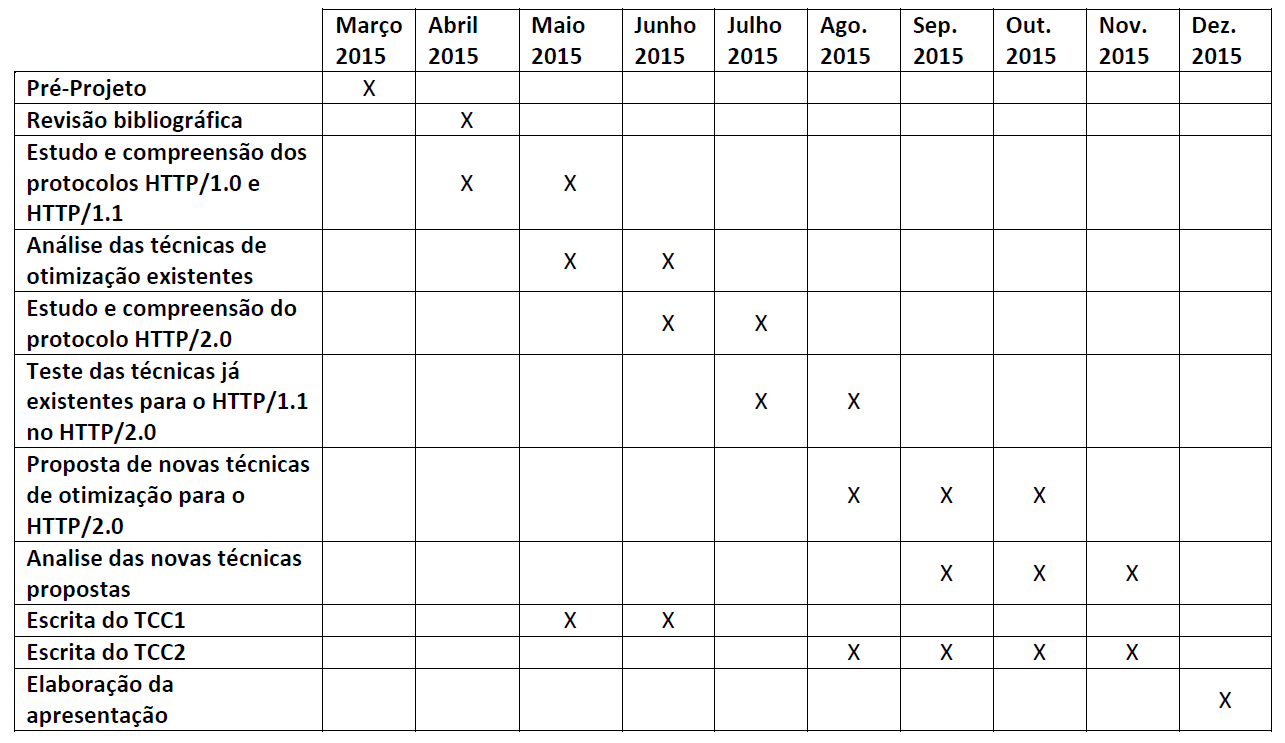
\includegraphics[width=1.0\textwidth]{./04-figuras/cronograma}
\end{quadro}           % Cronograma

    % Elementos pós textuais
    \postextual
    %
% Documento: Referências Bibliográficas
%

\bibliography{./refbase}    % Geração automática das referências por meio do arquivo 'refbase.bib'
       % Referências

    \printindex                                             % Índice remissivo

\end{document}
